% Options for packages loaded elsewhere
\PassOptionsToPackage{unicode}{hyperref}
\PassOptionsToPackage{hyphens}{url}
\PassOptionsToPackage{dvipsnames,svgnames,x11names}{xcolor}
%
\documentclass[
  letterpaper,
  DIV=11,
  numbers=noendperiod]{scrartcl}

\usepackage{amsmath,amssymb}
\usepackage{iftex}
\ifPDFTeX
  \usepackage[T1]{fontenc}
  \usepackage[utf8]{inputenc}
  \usepackage{textcomp} % provide euro and other symbols
\else % if luatex or xetex
  \usepackage{unicode-math}
  \defaultfontfeatures{Scale=MatchLowercase}
  \defaultfontfeatures[\rmfamily]{Ligatures=TeX,Scale=1}
\fi
\usepackage{lmodern}
\ifPDFTeX\else  
    % xetex/luatex font selection
\fi
% Use upquote if available, for straight quotes in verbatim environments
\IfFileExists{upquote.sty}{\usepackage{upquote}}{}
\IfFileExists{microtype.sty}{% use microtype if available
  \usepackage[]{microtype}
  \UseMicrotypeSet[protrusion]{basicmath} % disable protrusion for tt fonts
}{}
\makeatletter
\@ifundefined{KOMAClassName}{% if non-KOMA class
  \IfFileExists{parskip.sty}{%
    \usepackage{parskip}
  }{% else
    \setlength{\parindent}{0pt}
    \setlength{\parskip}{6pt plus 2pt minus 1pt}}
}{% if KOMA class
  \KOMAoptions{parskip=half}}
\makeatother
\usepackage{xcolor}
\setlength{\emergencystretch}{3em} % prevent overfull lines
\setcounter{secnumdepth}{-\maxdimen} % remove section numbering
% Make \paragraph and \subparagraph free-standing
\makeatletter
\ifx\paragraph\undefined\else
  \let\oldparagraph\paragraph
  \renewcommand{\paragraph}{
    \@ifstar
      \xxxParagraphStar
      \xxxParagraphNoStar
  }
  \newcommand{\xxxParagraphStar}[1]{\oldparagraph*{#1}\mbox{}}
  \newcommand{\xxxParagraphNoStar}[1]{\oldparagraph{#1}\mbox{}}
\fi
\ifx\subparagraph\undefined\else
  \let\oldsubparagraph\subparagraph
  \renewcommand{\subparagraph}{
    \@ifstar
      \xxxSubParagraphStar
      \xxxSubParagraphNoStar
  }
  \newcommand{\xxxSubParagraphStar}[1]{\oldsubparagraph*{#1}\mbox{}}
  \newcommand{\xxxSubParagraphNoStar}[1]{\oldsubparagraph{#1}\mbox{}}
\fi
\makeatother


\providecommand{\tightlist}{%
  \setlength{\itemsep}{0pt}\setlength{\parskip}{0pt}}\usepackage{longtable,booktabs,array}
\usepackage{calc} % for calculating minipage widths
% Correct order of tables after \paragraph or \subparagraph
\usepackage{etoolbox}
\makeatletter
\patchcmd\longtable{\par}{\if@noskipsec\mbox{}\fi\par}{}{}
\makeatother
% Allow footnotes in longtable head/foot
\IfFileExists{footnotehyper.sty}{\usepackage{footnotehyper}}{\usepackage{footnote}}
\makesavenoteenv{longtable}
\usepackage{graphicx}
\makeatletter
\newsavebox\pandoc@box
\newcommand*\pandocbounded[1]{% scales image to fit in text height/width
  \sbox\pandoc@box{#1}%
  \Gscale@div\@tempa{\textheight}{\dimexpr\ht\pandoc@box+\dp\pandoc@box\relax}%
  \Gscale@div\@tempb{\linewidth}{\wd\pandoc@box}%
  \ifdim\@tempb\p@<\@tempa\p@\let\@tempa\@tempb\fi% select the smaller of both
  \ifdim\@tempa\p@<\p@\scalebox{\@tempa}{\usebox\pandoc@box}%
  \else\usebox{\pandoc@box}%
  \fi%
}
% Set default figure placement to htbp
\def\fps@figure{htbp}
\makeatother
% definitions for citeproc citations
\NewDocumentCommand\citeproctext{}{}
\NewDocumentCommand\citeproc{mm}{%
  \begingroup\def\citeproctext{#2}\cite{#1}\endgroup}
\makeatletter
 % allow citations to break across lines
 \let\@cite@ofmt\@firstofone
 % avoid brackets around text for \cite:
 \def\@biblabel#1{}
 \def\@cite#1#2{{#1\if@tempswa , #2\fi}}
\makeatother
\newlength{\cslhangindent}
\setlength{\cslhangindent}{1.5em}
\newlength{\csllabelwidth}
\setlength{\csllabelwidth}{3em}
\newenvironment{CSLReferences}[2] % #1 hanging-indent, #2 entry-spacing
 {\begin{list}{}{%
  \setlength{\itemindent}{0pt}
  \setlength{\leftmargin}{0pt}
  \setlength{\parsep}{0pt}
  % turn on hanging indent if param 1 is 1
  \ifodd #1
   \setlength{\leftmargin}{\cslhangindent}
   \setlength{\itemindent}{-1\cslhangindent}
  \fi
  % set entry spacing
  \setlength{\itemsep}{#2\baselineskip}}}
 {\end{list}}
\usepackage{calc}
\newcommand{\CSLBlock}[1]{\hfill\break\parbox[t]{\linewidth}{\strut\ignorespaces#1\strut}}
\newcommand{\CSLLeftMargin}[1]{\parbox[t]{\csllabelwidth}{\strut#1\strut}}
\newcommand{\CSLRightInline}[1]{\parbox[t]{\linewidth - \csllabelwidth}{\strut#1\strut}}
\newcommand{\CSLIndent}[1]{\hspace{\cslhangindent}#1}

\KOMAoption{captions}{tablesignature}
\makeatletter
\@ifpackageloaded{caption}{}{\usepackage{caption}}
\AtBeginDocument{%
\ifdefined\contentsname
  \renewcommand*\contentsname{Table of contents}
\else
  \newcommand\contentsname{Table of contents}
\fi
\ifdefined\listfigurename
  \renewcommand*\listfigurename{List of Figures}
\else
  \newcommand\listfigurename{List of Figures}
\fi
\ifdefined\listtablename
  \renewcommand*\listtablename{List of Tables}
\else
  \newcommand\listtablename{List of Tables}
\fi
\ifdefined\figurename
  \renewcommand*\figurename{Figure}
\else
  \newcommand\figurename{Figure}
\fi
\ifdefined\tablename
  \renewcommand*\tablename{Table}
\else
  \newcommand\tablename{Table}
\fi
}
\@ifpackageloaded{float}{}{\usepackage{float}}
\floatstyle{ruled}
\@ifundefined{c@chapter}{\newfloat{codelisting}{h}{lop}}{\newfloat{codelisting}{h}{lop}[chapter]}
\floatname{codelisting}{Listing}
\newcommand*\listoflistings{\listof{codelisting}{List of Listings}}
\makeatother
\makeatletter
\makeatother
\makeatletter
\@ifpackageloaded{caption}{}{\usepackage{caption}}
\@ifpackageloaded{subcaption}{}{\usepackage{subcaption}}
\makeatother

\usepackage{bookmark}

\IfFileExists{xurl.sty}{\usepackage{xurl}}{} % add URL line breaks if available
\urlstyle{same} % disable monospaced font for URLs
\hypersetup{
  pdftitle={Using Cellular Communication Sensing to Support Early Recovery from Alcohol Use Disorder},
  pdfauthor={Kendra Wyant; Coco Yu; John J. Curtin},
  pdfkeywords={Substance use disorders, Machine learning, Cellular
Sensing},
  colorlinks=true,
  linkcolor={blue},
  filecolor={Maroon},
  citecolor={Blue},
  urlcolor={Blue},
  pdfcreator={LaTeX via pandoc}}


\title{Using Cellular Communication Sensing to Support Early Recovery
from Alcohol Use Disorder}
\author{Kendra Wyant \and Coco Yu \and John J. Curtin}
\date{2025-10-16}

\begin{document}
\maketitle


\textsubscript{Source:
\href{https://jjcurtin.github.io/study_messages/index.qmd.html}{Article
Notebook}}

\section{Introduction}\label{introduction}

Alcohol Use Disorder (AUD) is a chronic, relapsing disease (Dennis \&
Scott, 2007; McLellan et al., 2000; Rounsaville, 2010). Lapses, single
episodes of alcohol use, and relapse, a full return to harmful drinking,
can occur at any point in recovery (Kirshenbaum et al., 2009; Nguyen et
al., 2020; Scott et al., 2005; Witkiewitz, 2011). As with other chronic
health conditions where symptoms fluctuate, sometimes unexpectedly,
sustained AUD recovery requires ongoing monitoring of lapse risk.

Machine learning--guided recovery systems may now assist with the
inherently difficult task of identifying when and why someone is at
increased risk. Personal sensing of densely sampled data from
individuals' day-to-day lives can provide the inputs necessary for
temporally dynamic lapse predictions (Mohr et al., 2017). Early models
using ecological momentary assessment data have achieved excellent
accuracy (Chih et al., 2014; Wyant et al., 2024, under review). Still,
questions remain about the long-term feasibility of self-report sensing
methods and whether new, important risk factors might emerge from
sensing methods that passively collect smartphone data without user
input.

Cellular communication sensing may be one promising method. It offers
the potential for greater temporal specificity in capturing fluctuations
in risk compared with self-report data. Collecting communication data in
near real time could allow an algorithm to detect potential triggers as
they occur, without prompting users to reflect on their feelings or
waiting for users to report about their environement at a later point.
For example, late night phone calls could indicate an emergency, ``drunk
dialing'', or other risk-relevant interactions, while an expanding or
shrinking social circle could be characterized by the number of unique
contacts someone has communicated with.

These data may become even more powerful when communication contacts are
contextualized with personal meaning for a given participant (e.g., Who
is this contact to them? How pleasant or unpleasant is a typical
interaction with them? Have they drank with them in the past?). In this
scenario, contextualized communication logs might reveal that the
late-night phone call was to a sponsor, or that the shrinking social
circle was due to reduced contact with people who are unsupportive of
their recovery.

In this study, we evaluated the performance of a machine learning model
that predicts the probability of a next-day lapse using contextualized
cellular communication data. We also describe the most important
features contributing to these predictions, with the goal of identifying
new, clinically meaningful features emerging from communication-based
sensing.

\section{Methods}\label{methods}

\subsection{Participants and
Procedure}\label{participants-and-procedure}

We recruited adults in early recovery from AUD in Madison, Wisconsin,
through print and digital advertisements and partnerships with treatment
centers. Eligibility criteria required that participants were age 18 or
older, able to read and write in English, had moderate to severe AUD
\footnote{(≥4 self-reported DSM-5 symptoms)}, had been abstinent from
alcohol for 1--8 weeks, were willing to use a single smartphone, and
were not exhibiting severe psychosis or paranoia.\footnote{Defined as
  scores \textgreater2.2 or 2.8, respectively, on the psychosis or
  paranoia scales of the Symptom Checklist--90 (Derogatis, L.R., 2000).}

Participants completed up to 5 study visits over approximately 3 months:
a screening visit, intake visit, and 3 monthly follow-up visits. At
screening we collected demographic information (age, sex at birth, race,
ethnicity, education, marital status, employment, and income) and
clinical characteristics (DSM-5 AUD symptom count, alcohol problems
(Hurlbut \& Sher, 1992), and presence of psychological symptoms
(Derogatis, L.R., 2000)). At intake we collected additional self-report
data on abstinence self-efficacy (McKiernan et al., 2011), craving
(Flannery et al., 1999), and recent recovery efforts. At each monthly
follow-up, we downloaded cellular communication metadata (voice calls
and SMS text message logs) from participants' smartphones. We identified
important contacts (i.e., individuals they had communicated with at
least twice by call or text in the past month) and asked 7 contextual
questions about these contacts.

While enrolled, participants completed 4 brief daily ecological
momentary assessments (7-10 questions). The first item assessed alcohol
use (date and time of any unreported drinking episodes). Lapse reports
were verified at follow-up visits using a timeline follow-back
interview. Additional sensing data streams and self-report measures were
collected for the parent grant. The full study protocol is available on
our Open Science Framework page (\url{https://osf.io/wgpz9/}).

We screened 192 participants. Of these, 169 enrolled and 154 completed
the first follow-up. Data from 10 participants were excluded due to loss
of abstinence goals, careless responding, or unusually low compliance.
The final analytic sample included 144 participants.

\subsection{Data Analysis Plan}\label{data-analysis-plan}

Our models predicted the probability of an alcohol lapse within a
24-hour window. Predictions were generated daily at 4 a.m., beginning on
participants' second study day and continuing for up to 3 months. In
total, there were 11,507 labeled prediction windows across all
participants.

Features were engineered from all available data up to the start of each
window.\footnote{We filtered the data to include only communications
  with known context prior to feature engineering.} The full model
included 406 features from cellular communication data plus 24 features
from baseline self-report measures. We also evaluated a comparison model
that used only the baseline features. Table~\ref{tbl-1} details the raw
predictors and feature engineering procedures.

Candidate model configurations differed by algorithm (elastic net,
random forest, XGBoost), outcome resampling method, and hyperparameter
values. The best configuration for each model was selected using 6
repeats of participant-grouped 5-fold cross-validation. Our performance
metric was area under the receiver operating curve (auROC). Folds were
stratified by a between-subject measure of our outcome (low lapsers: 0-9
lapses; high lapsers: 10+ lapses).

We evaluated model performance with a Bayesian hierarchical generalized
linear model. Posterior distributions with 95\% credible intervals (CI)
were estimated from the 30 held-out test sets using weakly informative,
data-dependent priors to regularize and reduce overfitting.\footnote{Residual
  SD \textasciitilde{} normal(0, exp(2)); intercept (centered
  predictors) \textasciitilde{} normal(2.3, 1.3); window-width contrasts
  \textasciitilde{} normal(0, 2.69); covariance \textasciitilde{}
  decov(1,1,1,1).} Random intercepts were included for repeat and fold
(nested within repeat). auROCs were logit-transformed and regressed on
model type to estimate the probability that model performances differed
systematically.

Our best performing models used an elastic net algorithm. We quantified
feature importance by examining the retained features (i.e., coefficient
value \textgreater{} 0) in the full model and ordering them by absolute
coefficient value. These values provide an estimate of the direction and
magnitude of association between each predictor and the outcome,
conditional on the other features retained. All our annotated analysis
scripts are publicly available on our study website
(\url{https://jjcurtin.github.io/study_messages/}).

\begin{longtable}[]{@{}llllrll@{}}

\toprule\noalign{}
Raw Predictor & Response Options & Feature Engineering & Scoring Epochs
& Total Features & Full Model & Baseline Model \\
\midrule\noalign{}
\endhead
\bottomrule\noalign{}
\endlastfoot
Originated & Incoming, outgoing & Difference and raw rate counts for
text messages and voice calls & 6, 12, 24, 48, 72, and 168 hours & 48 &
Yes & No \\
Call duration & Duration (in minutes) & Difference and raw rate sums of
duration, difference and raw most recent duration & 6, 12, 24, 48, 72,
and 168 hours & 14 & Yes & No \\
Call answered & Yes, no & Difference and raw rate counts for unanswered
incoming voice calls & 6, 12, 24, 48, 72, and 168 hours & 12 & Yes &
No \\
Date/time of communication & Date and time & Difference and raw rate
counts for text messages and voice calls at night (10 pm -- 6am) and on
weekends & 24, 48, 72, and 168 hours (night), 168 hours (weekend) & 20 &
Yes & No \\
Phone number & Phone number & Difference and raw rate counts of unique
phone numbers & 6, 12, 24, 48, 72, and 168 hours & 12 & Yes & No \\
Type of Relationship & Family, friend, counselor or social worker,
co-worker & Difference and raw rate counts of unique phone numbers & 6,
12, 24, 48, 72, and 168 hours & 48 & Yes & No \\
Have you drank alcohol with this person? & Never/almost never,
occasionally, almost always/always & Difference and raw rate counts of
each response option & 6, 12, 24, 48, 72, and 168 hours & 36 & Yes &
No \\
What is their drinking status? & Drinker, non-drinker, don't know &
Difference and raw rate counts of each response option & 6, 12, 24, 48,
72, and 168 hours & 36 & Yes & No \\
Would you expect them to drink in your presence? & Yes, no, uncertain &
Difference and raw rate counts of each response option & 6, 12, 24, 48,
72, and 168 hours & 36 & Yes & No \\
Are they currently in recovery from drugs or alcohol? & Yes, no, don't
know & Difference and raw rate counts of each response option & 6, 12,
24, 48, 72, and 168 hours & 36 & Yes & No \\
Are they supportive about your recovery goals? & Supportive,
unsupportive, mixed, neutral, don't know & Difference and raw rate
counts of each response option & 6, 12, 24, 48, 72, and 168 hours & 60 &
Yes & No \\
How are your typical experiences with this person? & Pleasant,
unpleasant, mixed, neutral & Difference and raw rate counts of each
response option & 6, 12, 24, 48, 72, and 168 hours & 48 & Yes & No \\
DSM-5 symptom count & Numeric (4-11) & & & 1 & Yes & Yes \\
Past year alcohol problems & Numeric (0-27) & & & 1 & Yes & Yes \\
Craving & Numeric (0-30) & & & 1 & Yes & Yes \\
Abstinence self-efficacy: Negative affect, social, physical, and craving
subscales & Numeric (0-20) & & & 4 & Yes & Yes \\
Number of individual alcohol counseling sessions attended (past 30 days)
& Numeric & & & 1 & Yes & Yes \\
Number of group alcohol counseling sessions attended (past 30 days) &
Numeric & & & 1 & Yes & Yes \\
Number of self-help group meetings attended (past 30 days) & Numeric & &
& 1 & Yes & Yes \\
Number of other mental health counseling sessions attended (past 30
days) & Numeric & & & 1 & Yes & Yes \\
Number of days in contact with supportive people (past 30 days) &
Numeric & & & 1 & Yes & Yes \\
Number of days in contact with unsupportive people (past 30 days) &
Numeric & & & 1 & Yes & Yes \\
Taken prescribed medication for alcohol use disorder (past 30 days) &
Yes, no & Dummy coded & & 1 & Yes & Yes \\
Taken prescribed medication for other mental health disorder (past 30
days) & Yes, no & Dummy coded & & 1 & Yes & Yes \\
Satisfaction with progress toward recovery goals (past 30 days) &
Numeric (0-4) & & & 1 & Yes & Yes \\
Confidence in abstinence ability (next 30 days) & Numeric (0-4) & & & 1
& Yes & Yes \\
Has a goal of abstinence & Yes, no, uncertain & Dummy coded & & 2 & Yes
& Yes \\
Age & Numeric (years) & & & 1 & Yes & Yes \\
Sex at birth & Male, female & Dummy coded & & 1 & Yes & Yes \\
Race & Non-Hispanic White, non-White and/or Hispanic & Dummy coded & & 1
& Yes & Yes \\
Education & High school or less, some college, college degree & Dummy
coded & & 2 & Yes & Yes \\
Income & Numeric (dollars) & & & 1 & Yes & Yes \\
Marital Status & Married, not married, other & Dummy coded & & 2 & Yes &
Yes \\


\caption{\label{tbl-1}Feature Engineering of Raw Predictors}

\tabularnewline
\end{longtable}

\textsubscript{Source:
\href{https://jjcurtin.github.io/study_messages/notebooks/mak_tables-preview.html\#cell-tbl-1}{Make
All Tables for Main Manuscript}}

\subsection{Ethical Considerations}\label{ethical-considerations}

All procedures were approved by the University of Wisconsin-Madison
Institutional Review Board (Study \#2015-0780). All participants
provided written informed consent.

\section{Results}\label{results}

\subsection{Participants}\label{participants}

Table~\ref{tbl-2} provides the demographic characterization of our
sample. We obtained a total of 375,912 contextualized communications
across participants. Participants had, on average, 2,610 communications
(range = 109-14,225). 56\% of participants reported at least one lapse.

\begin{longtable}[]{@{}lrrlll@{}}

\toprule\noalign{}
& N & \% & M & SD & Range \\
\midrule\noalign{}
\endhead
\midrule\noalign{}
{Note: } & & & & & \\
\textsuperscript{} N = 144 & & & & & \\
\bottomrule\noalign{}
\endlastfoot
Age & & & 40.4 & 11.8 & 21-72 \\
Sex at Birth & & & & & \\
\multicolumn{6}{@{}l@{}}{%
\textbf{}} \\
Female & 74 & 51.4 & & & \\
Male & 70 & 48.6 & & & \\
Race & & & & & \\
\multicolumn{6}{@{}l@{}}{%
\textbf{}} \\
American Indian/Alaska Native & 3 & 2.1 & & & \\
Asian & 2 & 1.4 & & & \\
Black/African American & 8 & 5.6 & & & \\
White/Caucasian & 125 & 86.8 & & & \\
Other/Multiracial & 6 & 4.2 & & & \\
Hispanic, Latino, or Spanish origin & & & & & \\
\multicolumn{6}{@{}l@{}}{%
\textbf{}} \\
Yes & 3 & 2.1 & & & \\
No & 141 & 97.9 & & & \\
Education & & & & & \\
\multicolumn{6}{@{}l@{}}{%
\textbf{}} \\
Less than high school or GED degree & 1 & 0.7 & & & \\
High school or GED & 14 & 9.7 & & & \\
Some college & 39 & 27.1 & & & \\
2-Year degree & 13 & 9.0 & & & \\
College degree & 55 & 38.2 & & & \\
Advanced degree & 22 & 15.3 & & & \\
Employment & & & & & \\
\multicolumn{6}{@{}l@{}}{%
\textbf{}} \\
Employed full-time & 70 & 48.6 & & & \\
Employed part-time & 25 & 17.4 & & & \\
Full-time student & 7 & 4.9 & & & \\
Homemaker & 1 & 0.7 & & & \\
Disabled & 7 & 4.9 & & & \\
Retired & 8 & 5.6 & & & \\
Unemployed & 15 & 10.4 & & & \\
Temporarily laid off, sick leave, or maternity leave & 3 & 2.1 & & & \\
Other, not otherwise specified & 8 & 5.6 & & & \\
Personal Income & & & \$35,050 & \$32,069 & \$0-200,000 \\
Marital Status & & & & & \\
\multicolumn{6}{@{}l@{}}{%
\textbf{}} \\
Never married & 63 & 43.8 & & & \\
Married & 32 & 22.2 & & & \\
Divorced & 42 & 29.2 & & & \\
Separated & 5 & 3.5 & & & \\
Widowed & 2 & 1.4 & & & \\


\caption{\label{tbl-2}Demographics}

\tabularnewline
\end{longtable}

\textsubscript{Source:
\href{https://jjcurtin.github.io/study_messages/notebooks/mak_tables-preview.html\#cell-tbl-2}{Make
All Tables for Main Manuscript}}

\subsection{Model Evaluation}\label{model-evaluation}

The median posterior auROC for the full model was 0.68, with relatively
narrow 95\% CI ({[}0.64, 0.71{]}) that did not contain .5. This provides
strong evidence that the model is capturing signal in the data. The
final model retained 13 features (Figure~\ref{fig-1}). The top four were
baseline measures of abstinence confidence, having a goal of abstinence,
abstinence self-efficacy when experiencing negative affect, and craving.
Communication frequency with people unaware of the individual's recovery
goals also emerged as an important feature associated with increased
lapse risk.

We evaluated a comparison model to assess the incremental predictive
value of cellular communication features beyond baseline measures. The
baseline model retained 5 features and achieved performance nearly
identical to the full model (median auROC = 0.68, 95\% CI {[}0.64,
0.71{]}). The median difference in auROC between the full and baseline
models was less than .01, providing no evidence (52\% probability) that
their posterior distributions were meaningfully different.

\begin{figure}[H]

\centering{

\pandocbounded{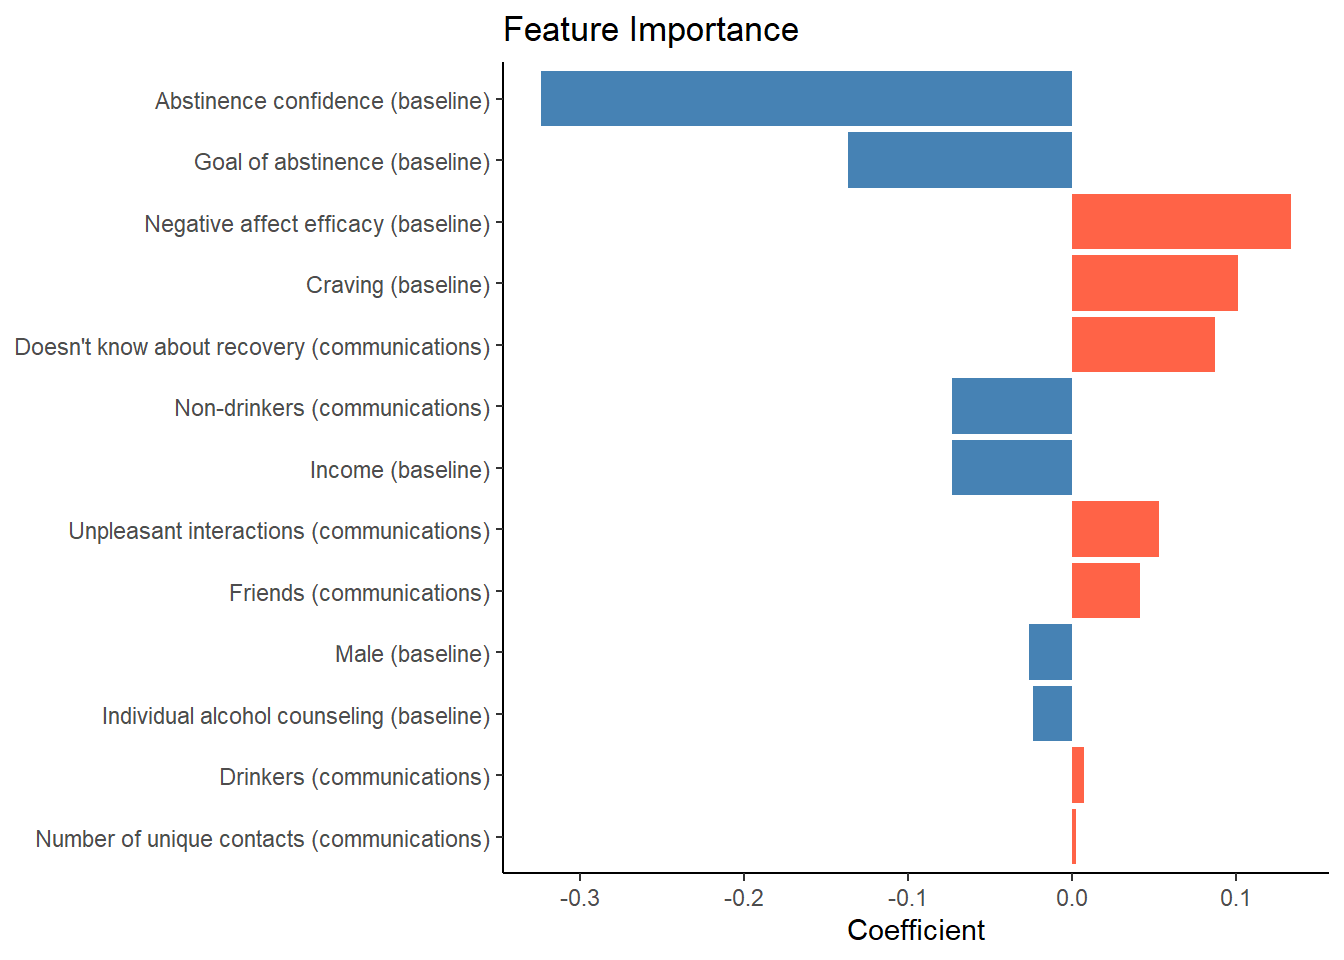
\includegraphics[keepaspectratio]{index_files/figure-latex/notebooks-mak_figures-fig-1-output-1.png}}

}

\caption{\label{fig-1}Global feature importance (elastic net
coefficient) for the full model. Features are ordered by absolute
coefficient value. Blue bars indicate higher feature values, on average,
lower lapse risk. Red bars indicate higher feature values, on average,
increase risk. Baseline features were collected from self-report
measures at the start of the study. Communication features were
engineered from the contexualized cellular communications.}

\end{figure}%

\textsubscript{Source:
\href{https://jjcurtin.github.io/study_messages/notebooks/mak_figures-preview.html\#cell-fig-1}{Make
All Figures for Main Manuscript}}

\section{Discussion}\label{discussion}

Our machine learning model incorporating cellular communications
achieved fair performance, with an auROC of 0.68, indicating that some
signal was present in the data. However, we found no incremental
predictive value compared to a baseline model that included only
demographic variables and self-report measures. In the full model, which
combined cellular communication and baseline measures, the four most
important predictors were all self-report variables: abstinence
confidence, abstinence goal, negative affect efficacy, and craving.

This finding suggests that cellular communication data may not add
substantial information for predicting lapse risk beyond what can
already be captured by brief self-report and demographic measures.
Nonetheless, it is notable that several communication features were
retained in the final model with moderately sized coefficients. These
features, including communications with people unaware of the
participant's recovery status, with non-drinkers, with friends, and with
individuals who were unpleasant to interact with, may still offer some
insight into lapse vulnerability.

In contrast, raw counts of calls and text messages and call durations
were not retained in the final model. This implies that the quantity of
communications alone may be less informative for lapse prediction than
the quality and social meaning of the interactions. Future research may
benefit from collecting richer contextual information about
communication contacts to better understand the social dynamics
contributing to lapse risk. Even with highly contextualized
communication data, however, prediction may be constrained by data
sparsity. Many participants had relatively few communications per day,
and some had extended periods with no recorded interactions at all. Such
sparsity limits the capacity of these data to capture short-term
fluctuations in lapse risk.

Our study design may have further contributed to this limitation. We
collected only phone and SMS text communications through the native
smartphone app. Yet, in recent years, many individuals have shifted
their primary communication to private messaging apps (e.g., WhatsApp,
Signal) or social media platforms (e.g., Facebook Messenger, Instagram)
(\textbf{mcdowellPreferencesAttitudesDigital2025?}). As a result, our
dataset likely did not capture the full range of participants' social
interactions. Future studies could examine whether communication data
from these platforms yield stronger predictive signal.

Overall, our findings suggest that models using passive cellular sensing
captured limited incremental signal for lapse prediction beyond
demographic and self-report measures. While we do not rule out the
potential value of cellular communication data in certain contexts, our
results underscore the need to explore other passive sensing methods,
such as geolocation, which may provide denser data that captures
different aspects of daily life relevant to lapse risk.

\newpage

\phantomsection\label{refs}
\begin{CSLReferences}{1}{0}
\bibitem[\citeproctext]{ref-chihPredictiveModelingAddiction2014}
Chih, M.-Y., Patton, T., McTavish, F. M., Isham, A. J., Judkins-Fisher,
C. L., Atwood, A. K., \& Gustafson, D. H. (2014). Predictive modeling of
addiction lapses in a mobile health application. \emph{Journal of
Substance Abuse Treatment}, \emph{46}(1), 29--35.
\url{https://doi.org/10.1016/j.jsat.2013.08.004}

\bibitem[\citeproctext]{ref-dennisManagingAddictionChronic2007}
Dennis, M., \& Scott, C. K. (2007).
\href{https://www.ncbi.nlm.nih.gov/pmc/articles/PMC2797101}{Managing
{Addiction} as a {Chronic Condition}}. \emph{Addiction Science \&
Clinical Practice}, \emph{4}(1), 45--55.

\bibitem[\citeproctext]{ref-derogatislBriefSymptomInventory}
Derogatis, L.R. (2000). \emph{Brief {Symptom Inventory} 18 -
{Administration}, scoring, and procedures manual}. NCS Pearson.

\bibitem[\citeproctext]{ref-flanneryPsychometricPropertiesPenn1999}
Flannery, B. A., Volpicelli, J. R., \& Pettinati, H. M. (1999).
\href{https://www.ncbi.nlm.nih.gov/pubmed/10470970}{Psychometric
properties of the {Penn Alcohol Craving Scale}}. \emph{Alcoholism,
Clinical and Experimental Research}, \emph{23}(8), 1289--1295.

\bibitem[\citeproctext]{ref-hurlbutAssessingAlcoholProblems1992}
Hurlbut, S. C., \& Sher, K. J. (1992). Assessing alcohol problems in
college students. \emph{Journal of American College Health.},
\emph{41}(2), 49--58.

\bibitem[\citeproctext]{ref-kirshenbaumQuantitativeReviewUbiquitous2009}
Kirshenbaum, A. P., Olsen, D. M., \& Bickel, W. K. (2009). A
quantitative review of the ubiquitous relapse curve. \emph{Journal of
Substance Abuse Treatment}, \emph{36}(1), 8--17.
\url{https://doi.org/10.1016/j.jsat.2008.04.001}

\bibitem[\citeproctext]{ref-mckiernanDevelopmentBriefAbstinence2011}
McKiernan, P., Cloud, R., Patterson, D. A., Wolf, S., Golder, S., \&
Besel, K. (2011). Development of a {Brief Abstinence Self-Efficacy
Measure}. \emph{Journal of Social Work Practice in the Addictions},
\emph{11}(3), 245--253.
\url{https://doi.org/10.1080/1533256X.2011.593445}

\bibitem[\citeproctext]{ref-mclellanDrugDependenceChronic2000}
McLellan, A. T., Lewis, D. C., O'Brien, C. P., \& Kleber, H. D. (2000).
Drug dependence, a chronic medical illness: Implications for treatment,
insurance, and outcomes evaluation. \emph{JAMA}, \emph{284}(13),
1689--1695. \url{https://doi.org/10.1001/jama.284.13.1689}

\bibitem[\citeproctext]{ref-mohrPersonalSensingUnderstanding2017}
Mohr, D. C., Zhang, M., \& Schueller, S. M. (2017). Personal {Sensing}:
{Understanding Mental Health Using Ubiquitous Sensors} and {Machine
Learning}. \emph{Annual Review of Clinical Psychology}, \emph{13}(1),
23--47. \url{https://doi.org/10.1146/annurev-clinpsy-032816-044949}

\bibitem[\citeproctext]{ref-nguyenPredictingRelapseAlcohol2020a}
Nguyen, L.-C., Durazzo, T. C., Dwyer, C. L., Rauch, A. A., Humphreys,
K., Williams, L. M., \& Padula, C. B. (2020). Predicting {Relapse After
Alcohol Use Disorder Treatment} in a {High-Risk Cohort}: {The Roles} of
{Anhedonia} and {Smoking}. \emph{Journal of Psychiatric Research},
\emph{126}, 1--7. \url{https://doi.org/10.1016/j.jpsychires.2020.04.003}

\bibitem[\citeproctext]{ref-rounsavilleLapseRelapseChasing2010}
Rounsaville, D. B. (2010). \emph{Lapse, {Relapse}, and {Chasing} the
{Wagon}: {Post-Treatment Drinking} and {Recovery}} {[}PhD thesis{]}.
University of Maryland, Baltimore County.

\bibitem[\citeproctext]{ref-scottPathwaysRelapseTreatment2005}
Scott, C. K., Foss, M. A., \& Dennis, M. L. (2005). Pathways in the
relapse--treatment--recovery cycle over 3 years. \emph{Journal of
Substance Abuse Treatment}, \emph{28 Suppl 1}, S63--72.
\url{https://doi.org/10.1016/j.jsat.2004.09.006}

\bibitem[\citeproctext]{ref-witkiewitzPredictorsHeavyDrinking2011}
Witkiewitz, K. (2011). Predictors of heavy drinking during and following
treatment. \emph{Psychology of Addictive Behaviors}, \emph{25}(3),
426--438. \url{https://doi.org/10.1037/a0022889}

\bibitem[\citeproctext]{ref-wyantForecastingRiskAlcoholunderreview}
Wyant, K., Fronk, G. E., Yu, C., Punturieri, C. E., \& Curtin, J. J.
(under review). \emph{Forecasting {Risk} of {Alcohol Lapse} up to {Two
Weeks} in {Advance} using {Time-lagged Machine Learning Models}}.

\bibitem[\citeproctext]{ref-wyantMachineLearningModels2024}
Wyant, K., Sant'Ana, S. J., Fronk, G. E., \& Curtin, J. J. (2024).
Machine learning models for temporally precise lapse prediction in
alcohol use disorder. \emph{Journal of Psychopathology and Clinical
Science}, \emph{133}(7), 527--540.
\url{https://doi.org/10.1037/abn0000901}

\end{CSLReferences}




\end{document}
